% !TeX spellcheck = en_US


\chapter{Hardware Design}


\section{Magnetically transduced whisker sensor}
The structure of a single whisker sensor is shown in \cref{fig:whisker_composite}.

\begin{figure}[ht]
    \centering
    \begin{subfigure}{0.31\textwidth}
        \centering
        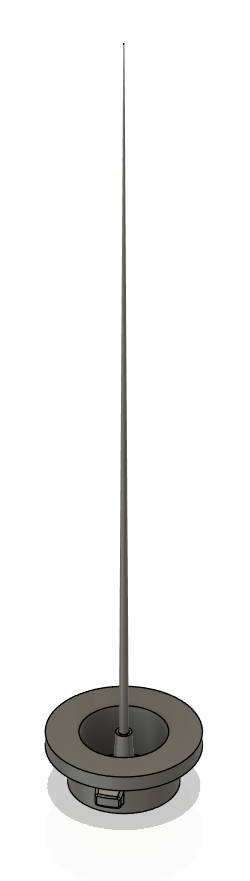
\includegraphics[height=0.2\textheight]{figures/whisker}
        \caption{Whisker mounted on the suspension} \label{fig:whisker}
    \end{subfigure}%
    \hspace*{\fill}   % maximize separation between the subfigures
    \begin{subfigure}{0.31\textwidth}
        \centering
        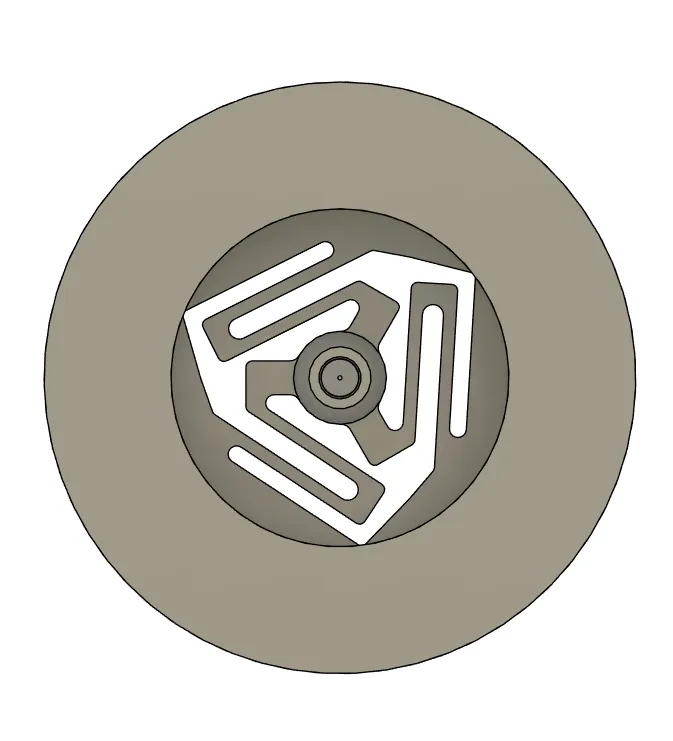
\includegraphics[width=\linewidth]{figures/suspension}
        \caption{Suspension Design} \label{fig:suspension}
    \end{subfigure}%
    \hspace*{\fill}   % maximizeseparation between the subfigures
    \begin{subfigure}{0.31\textwidth}
        \centering
        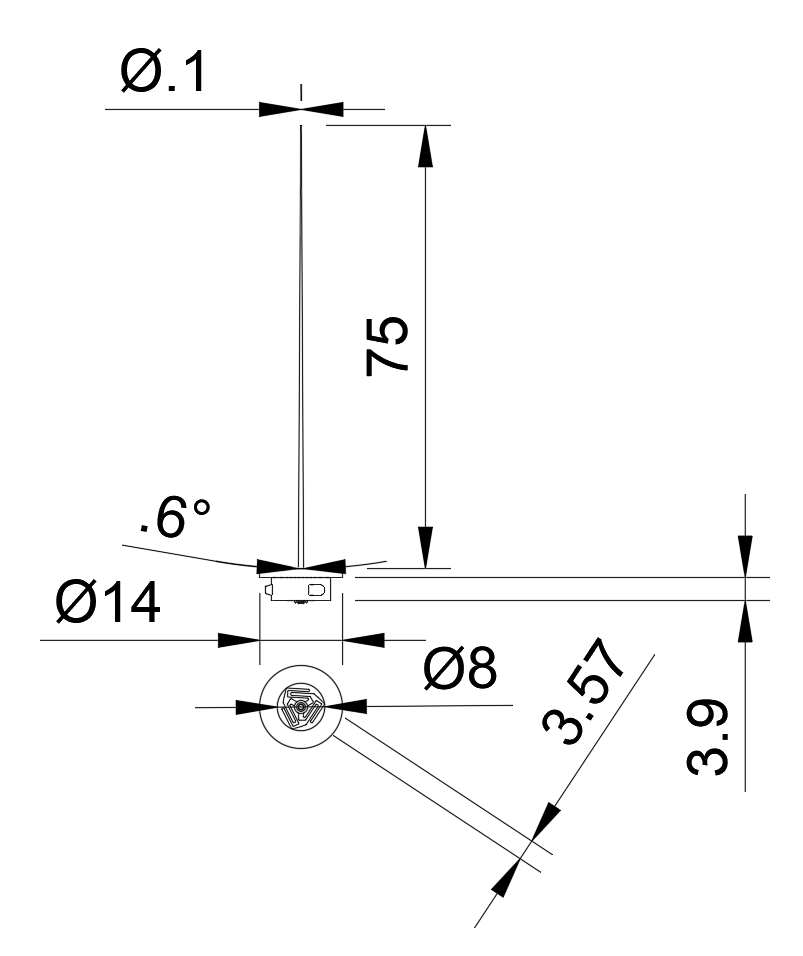
\includegraphics[width=\linewidth]{figures/whisker-dims}
        \caption{Structure dimensions} \label{fig:whisker-dims}
    \end{subfigure}
    \caption{Single whisker sensor.}
    \label{fig:whisker_composite}
\end{figure}

The whisker consists of:
\begin{itemize}
    \item A flexible whisker shaft made of a nitinol wire (0.25 mm diameter, 75 mm length).
    \item A suspension system fabricated via 3D printing using PLA plastic as filament.
    \item A magnetic sensor Adafruit MLX90393, configured for measuring magnetic flux changes with resolution of 0.15 $\micro T/LSB$
\end{itemize}
The whisker shaft is first glued to the suspension system.
A neodymium permanent magnet, axially magnetized with its field direction aligned with the wire, is placed underneath.
The suspension hooks are designed to allow screwing in the whiskers into the whisker mount.

\section{Whisker Platform}

A whisker platform was developed integrate multiple whisker sensors simultaneously.
It consists of a triangularly-shaped body, two side clamps, which allow for 3 whiskers to be attached on each side, and a mount for the Franka Panda robotic arm.
The platform has a size of 90 mm x 60 mm x 35 mm and is 3D printed using PLA plastic filament.
Six whiskers are attached at a 3D-printed PLA-platform, 3 per each side, as shown in \cref{fig:whisker_platform}.
Additionally, a mount for the Franke Panda robotic arm was designed to allow the whisker platform to be moved and rotated.

\begin{figure}[ht]
    \centering
    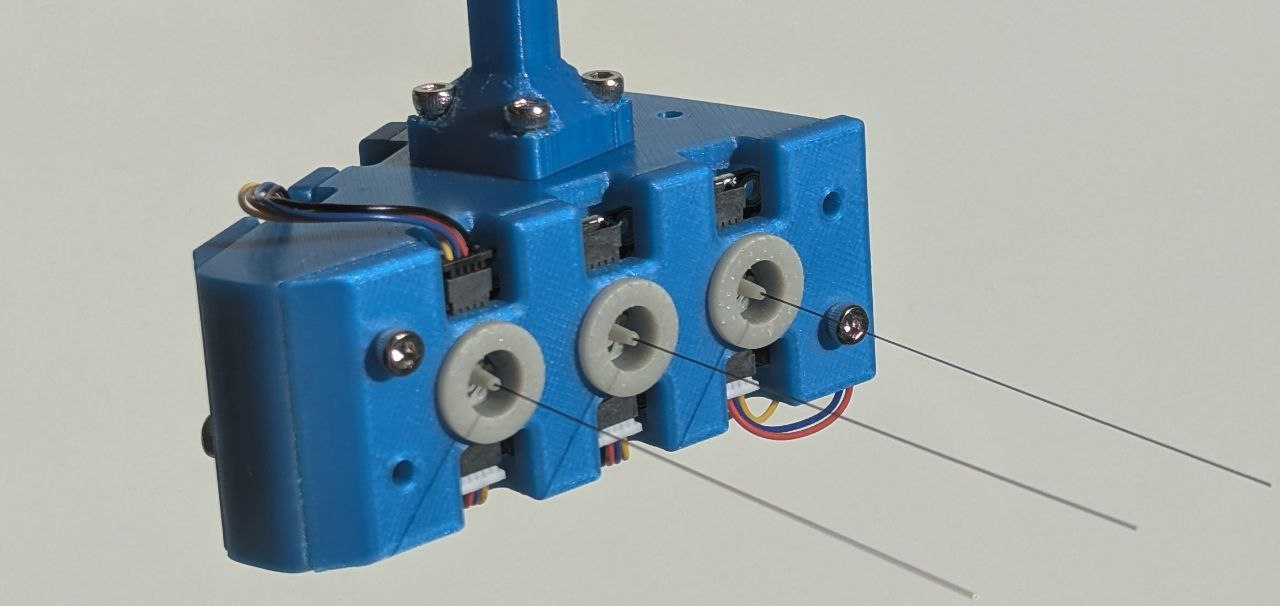
\includegraphics[width=0.8\textheight]{figures/platform}
    \caption{Whisker platform with three whisker attached to the left side and robotic arm mount at the top.}
    \label{fig:whisker_platform}
\end{figure}

\section{Data Acquisition}
...

